\documentclass[11pt]{article}

\usepackage{listings}
\usepackage{graphicx}

\begin{document}
\title{%
  Diffusion Limited Aggregation \\
  \large Simulating the Formation of Biological Crystal \\
  Growth in Flud Systems}
\author{Jarred Parr}

\date{October 2018}
\maketitle

\section{Introduction}
The following writeup outlines the process an conclusions gathered from studying diffusion limited aggregation in biological systems. Its goal was to simulate the formation of crystals in any number of naturally occuring situations like gout, battery corrosion, and even snowflakes.

\section{Program Architecture}
All simulation code was abstracted from the main file in order to facilitate additional functionality as needed. Classes were also used to better group functionality. An initial attempt at writing this simulation led me to consider a class based approach of particle management. In it I had things like internal state management and point tracking, but that was in the idea of implementing a more fully featured and robust simulation. Due to time constraints, this unfortunately didn't get too far off of the ground.

I took two main considerations in my code design:
\begin{itemize}
  \item Function
  \item Form
\end{itemize}

The code needed to work before significant refactoring could take place to remove issues like redundant code and to handle some of the more intricate features of the code. In the idea of function, I took as strongly of a functional programming approach to this problem as I could. This allowed me the flexibility to write my code in a more loosely coupled fashion while also being able to preserve the speed gains of using C++. The parallelism was largely applied in the use of the main loops in the code. When used elsewhere it made for an extreme amount of issues and bottlenecks when accessing the values due to the neeed for crical and atomic pragma uses. That being said, I now firmly know that there is such a thing as too much parallelism.

\section{Results}
\begin{figure}[h!]
  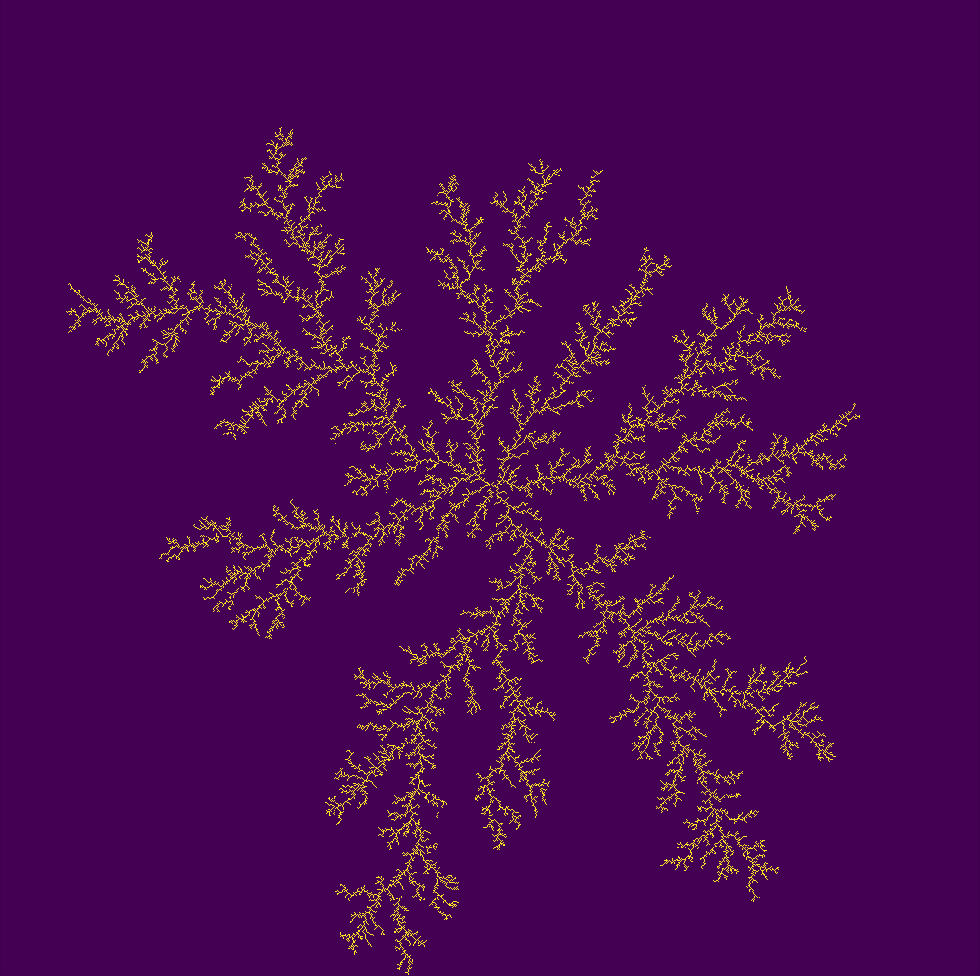
\includegraphics[width=\linewidth]{output.png}
  \caption{The generated structure}
\end{figure}
\begin{figure}[h!]
  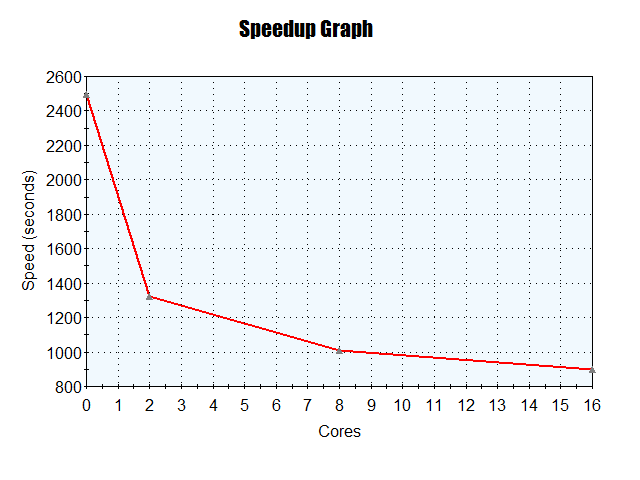
\includegraphics[width=\linewidth]{speedup.png}
  \caption{The speedup graph}
\end{figure}
The code strongly exihibited the law of diminishing marginal returns. As shown below, as the number of cores increased, the linear speedup began to level off and saw only marginal gains as the number of cores increased. This has led me to hypothesize that had the number of parallel threads increased, the speed of exection would have continued to see smaller and smaller improvements from run-to-run.

The following results are for a 10 million particle 10,000 by 10,000 grid

\begin{itemize}
  \item Sequential: 2496s
  \item 2 Core: 1325s
  \item 8 Core: 1008s
  \item 16 Core: 896s
\end{itemize}


All of these times were the peak running times of 8 repeated attempts each which was handled via bash script automation.

\section{Source Code}
My full source code for the crystal.cc class, where 99\% of the logic is, is as follows:

\lstset{frame=tb,
  language=C++
}

\begin{lstlisting}
#include <algorithm>
#include <chrono>
#include <crystal/crystal.hpp>
#include <fstream>
#include <iostream>
#include <iterator>
#include <random>
#include <omp.h>

namespace crystal {
  auto read_simulation_space = [](
      const int64_t x,
      const int64_t y,
      const std::vector<std::vector<int>>& simulation_space)->int {
    int val = 0;
    #pragma omp atomic read
    val = simulation_space[x][y];
    return val;
  };

  auto write_simulation_space = [](
      const int64_t x,
      const int64_t y,
      std::vector<std::vector<int>>& simulation_space, int val)->void {
    #pragma omp atomic write
    simulation_space[x][y] = val;
  };

  auto read_radius = [](const int& radius)->int {
    int val = 0;
    #pragma omp atomic read
    val = radius;
    return val;
  };

  auto write_radius = [](int& radius, int val)->void {
    #pragma omp atomic write
    radius = val;
  };

  Crystal::Crystal(int64_t particles, int64_t simulation_size) {
    this->SIMULATION_SIZE = simulation_size;
    this->ROWS = simulation_size;
    this->COLS = simulation_size;
    this->MAX_MOVES = 4 * simulation_size;
    this->CENTER = simulation_size / 2;
  }

  void Crystal::Run(int64_t particles) {
    int radius = 0;
    std::vector<std::vector<int>> simulation_space(
        this->ROWS,
        std::vector<int>(this->COLS));

    // Place our point in the center of the board
    simulation_space[this->CENTER][this->CENTER] = 1;
    omp_set_num_threads(16);

    auto now = std::chrono::high_resolution_clock::now();
    #pragma omp parallel
    {
      for (int i = 0; i < particles; ++i) {
        if (read_radius(radius) >= this->SIMULATION_SIZE / 2) {
          continue;;
        }

        const auto point_location = this->insert_particle(
					simulation_space,
					radius);
        int64_t x = std::get<0>(point_location);
        int64_t y = std::get<1>(point_location);
        this->random_walk(x, y, simulation_space);

        if (x >= 0 &&
            x < this->SIMULATION_SIZE &&
            y >= 0 && y < this->SIMULATION_SIZE) {
          const int distance = std::max(std::abs(
          this->CENTER - x), std::abs(this->CENTER - y));

          if (distance > read_radius(radius)) {
            write_radius(radius, distance);
          }
        }

        this->end_simulation(simulation_space);
      }
    }
    auto end = std::chrono::high_resolution_clock::now();

    std::cout << std::chrono::duration_cast<std::chrono::seconds>(end - now).count() << "s" << std::endl;
  }

  void Crystal::end_simulation(const std::vector<std::vector<int>> &simulation_space) {
    std::ofstream the_goods;

    the_goods.open("output.txt");

    for (uint64_t i = 0; i < simulation_space.size(); ++i) {
      for (uint64_t j = 0; j < simulation_space[i].size(); ++j) {
        int current = 0;

        if (simulation_space[i][j] == 1) {
          current = 1;
        }

        if (j != 0) {
          the_goods << " ";
        }

        the_goods << current;
      }
      the_goods << "\n";
    }

    the_goods.close();
  }

  void Crystal::print(
		const std::vector<std::vector<int>>& simulation_space
		) {
    for (uint64_t i = 0; i < this->SIMULATION_SIZE; ++i) {
      for (uint64_t j = 0; j < this->SIMULATION_SIZE; ++j) {
        int current = simulation_space[i][j];

        std::cout << current << ", " << std::endl;
      }

      std::cout << "\n" << std::endl;
    }
  }

  void Crystal::random_walk(
      int64_t &x,
      int64_t &y,
      std::vector<std::vector<int>> &simulation_space
      ) {
    std::random_device rd;
    std::mt19937 g(rd());

    while (x >= 0 &&
					 x < this->SIMULATION_SIZE &&
           y >= 0 && y < this->SIMULATION_SIZE) {
      if (this->collision(x, y, simulation_space)) {
        std::cout << "Writing to simulation space!" << std::endl;
        write_simulation_space(x, y, simulation_space, 1);
        return;
      }

      x += g() % 2;
      y += g() % 2;
    }
}

  bool Crystal::collision(
    int64_t x,
    int64_t y,
    const std::vector<std::vector<int>>& simulation_space) {
    for (int i = -1; i <= 1; i++) {
      for (int j = -1; j <= 1; j++) {
        const int64_t t_x = x + i;
        const int64_t t_y = y + j;

        if (t_x >= 0 && t_x < this->SIMULATION_SIZE &&
            t_y >= 0 && t_y < this->SIMULATION_SIZE &&
            read_simulation_space(t_x, t_y, simulation_space) == 1) {
            return true;
        }
      }
    }

    return false;
  }

  std::tuple<int64_t, int64_t> Crystal::insert_particle(
      const std::vector<std::vector<int>>& simulation_space,
      const int radius
      ) {
    std::random_device rd;
    std::mt19937 g(rd());
    std::uniform_int_distribution<int64_t> uni(0, this->SIMULATION_SIZE - 1);
    int64_t random_row = 0;
    int64_t random_col = 0;

    do {
      random_row = uni(g);
      random_col = uni(g);
      std::cout << random_row << std::endl;
      std::cout << random_col << std::endl;
    } while ((abs(this->CENTER - random_row) <= radius + 1 &&
              abs(this->CENTER - random_col) <= radius - 1) ||
              read_simulation_space(random_row, random_col, simulation_space) != 0);

    return std::make_tuple(random_row, random_col);
  }

}// namespace crystal
\end{lstlisting}

\section{Conclusion}
Overall this project has taught me a lot about the fine line between truly optimized code and over optimization. I feel like I have a much better understanding of openmp and the work is does to run the code in parallel. For awhile it felt so easily to simply place a \#pragma omp call all over the place and expect an extremely speedy program, but I have since learned that this is just not the case. Overall my code was able to exhibit a speedup of about 3. Given the circumstances and the time constraint I believe I could have optimized it further, but with other project deadlines and other situtaions arising it was difficult to put in an extreme amount of time towards squeezing every last piece of performance out of this project. So I will take what I can get and use it as a stepping stone to move forward. Simulations have always interested me and I am very happy to be able to have explored them in some capacity with this project.

\end{document}
